Chương này tập trung làm rõ hành vi của chương trình, độ tương tự về
hành vi giữa hai chương trình. Ngoài ra, chương này còn trình bày một 
số kiến thức cơ sở về kiểm thử phần mềm và kỹ thuật sinh dữ liệu kiểm 
thử trong Phần \ref{sec:base}.
\section{Kiến thức cơ sở}
\label{sec:base}

Ý tưởng chính của việc đo độ tương tự về hành vi giữa hai chương trình
máy tính là dựa trên tập dữ liệu vào, đếm số lượng dữ liệu ra tương
ứng giống nhau giữa hai chương trình và đo tỷ lệ tương tự. Dữ liệu vào
phải được chọn sao cho phủ nhiều nhất miền vào của chương trình. Về cơ
bản, độ tương tự này được đo dựa trên dữ liệu các ca kiểm thử. Chương
này trình bày ngắn gọn về kiểm thử phần mềm cùng việc sinh dữ liệu
kiểm thử, chủ yếu tập trung vào phương pháp thực thi biểu trưng một
chương trình (\emph{DSE -- Dynamic Symbolic Execution}) nhằm giúp 
tăng độ phủ của dữ liệu thử.

\subsection{Kiểm thử phần mềm}
Hiện nay, ngành công nghiệp phần mềm giữ vai trò khá quan trọng. Một
số nước có nền công nghệ thông tin phát triển thì ngành công nghiệp
phần mềm có khả năng chi phối cả nền kinh tế. Vì vậy, việc đảm bảo
chất lượng phần mềm trở nên cần thiết hơn bao giờ hết.

Quá trình phát hiện và khắc phục lỗi của phần mềm là một công việc đòi 
hỏi nhiều nỗ lực, công sức, phát sinh thêm nhiều chi phí trong việc phát 
triển phần mềm. Một sản phẩm phần mềm đạt chất lượng, đáp ứng được yêu 
cầu của người sử dụng sẽ được nhiều người biết đến, nó mang lại hiệu quả 
tích cực trong công việc của người sử dụng. Ngược lại, một phần mềm kém 
chất lượng sẽ gây thiệt hại về kinh tế, ảnh hưởng đến công việc của người 
sử dụng. Vì vậy, yêu cầu đặt ra đó là một sản phẩm phần mềm phải đảm bảo 
được sự ổn định, không phát sinh lỗi trong quá trình sử dụng.

Kiểm thử phần mềm chính là một quá trình hoặc một loạt các quy trình
được thiết kế nhằm đảm bảo mã máy tính chỉ làm những gì nó được thiết
kế và không làm bất cứ điều gì ngoài ý muốn \cite{myers2011art}. Đây
là một bước quan trọng trong quá trình phát triển một phần mềm, giúp
cho nhà phát triển phần mềm và người sử dụng thấy được hệ thống đã đáp
ứng được yêu cầu đặt ra.

\subsubsection*{Các phương pháp kiểm thử}

Có nhiều phương pháp để kiểm thử phần mềm, trong đó hai phương pháp
kiểm thử chính là \emph{kiểm thử tĩnh} và \emph{kiểm thử động}.

\emph{Kiểm thử tĩnh (Static testing)} là phương pháp kiểm thử phần mềm
bằng cách duyệt lại các yêu cầu, các đặc tả và mã lệnh chương trình
bằng tay, thông qua việc sử dụng giấy, bút để kiểm tra tính logic từng
chi tiết mà không cần chạy chương trình. Kiểu kiểm thử này thường được
sử dụng bởi chuyên viên thiết kế, người viết mã lệnh chương
trình. Kiểm thử tĩnh cũng có thể được tự động hóa bằng cách thực hiện
kiểm tra toàn bộ hệ thống thông qua một trình thông dịch hoặc trình
biên dịch, xác nhận tính hợp lệ về cú pháp của chương trình.
		
\emph{Kiểm thử động (Dynamic testing)} là phương pháp kiểm thử thông
qua việc thực thi chương trình để kiểm tra trạng thái tác động của
chương trình, dựa trên các ca kiểm thử xác định các đối tượng kiểm thử
của chương trình. Đồng thời, kiểm thử động sẽ tiến hành kiểm tra cách
thức hoạt động của mã lệnh, tức là kiểm tra phản ứng từ hệ thống với
các biến thay đổi theo thời gian. Trong kiểm thử động, phần mềm phải
được biên dịch và chạy, và bao gồm việc nhập các giá trị đầu vào và
kiểm tra các giá trị đầu ra.

Trong luận văn này, độ tương tự về hành vi giữa hai chương trình được
đo thông qua việc thực thi hai chương trình, tức là sử dụng phương
pháp \emph{kiểm thử động}.
	
\subsubsection*{Các chiến lược kiểm thử}

Hai chiến lược kiểm thử phần mềm được sử dụng nhiều nhất đó là 
\emph{kiểm thử hộp đen} và \emph{kiểm thử hộp trắng}.
	
\emph{Kiểm thử hộp đen – black box} là một chiến lược kiểm thử với
cách thức hoạt động chủ yếu dựa vào hướng dữ liệu inputs/outputs của
chương trình, xem chương trình như là một ``hộp đen''. Chiến lược kiểm
thử này hoàn toàn không quan tâm về cách xử lý và cấu trúc bên trong
của chương trình, nó tập trung vào tìm các trường hợp mà chương trình
không thực hiện theo các đặc tả. Tuy nhiên, phương pháp kiểm thử này
cũng có mặt hạn chế của nó, kiểm thử viên không biết các phần mềm cần
kiểm tra thực sự được xây dựng như thế nào, cố gắng viết rất nhiều ca
kiểm thử để kiểm tra một chức năng của phần mềm nhưng lẽ ra chỉ cần
kiểm tra bằng một vài ca kiểm thử, một số phần của chương trình
có thể sẽ bị bỏ qua không được kiểm tra.

Do vậy, kiểm thử hộp đen có ưu điểm là đánh giá khách quan, mặt khác
nó lại có nhược điểm là thăm dò mù. Trong phần nghiên cứu của đề tài,
kiểm thử hộp đen cũng được sử dụng như một phương pháp đo độ tương tự
hành vi của các chương trình.
		
\emph{Kiểm thử hộp trắng (white box)} là một chiến lược kiểm ngược lại
với kiểm thử hộp đen, còn gọi là kiểm thử hướng logic của phần
mềm. Cách kiểm thử này cho phép tạo ra dữ liệu thử nghiệm từ việc kiểm
tra, khảo sát cấu trúc bên trong và kiểm thử tính logic của chương
trình. Dữ liệu thử nghiệm có độ phủ lớn, đảm bảo tất cả các đường dẫn,
hoặc các nhánh của chương trình được thực hiện ít nhất một lần, khắc
phục được nhược điểm thăm dò mù trong cách kiểm thử hộp đen.			

\subsection{Kỹ thuật Dynamic symbolic execution}
\label{sec:dse}

Dynamic symbolic execution (DSE) là một kỹ thuật sinh dữ liệu thử bằng
cách duyệt tự động tất cả các đường đi có thể của chương trình, chạy 
chương trình với nhiều giá trị đầu vào khác nhau để tăng độ
phủ của dữ liệu thử \cite{xie2009fitness,cadar2013symbolic}.

Dựa trên kiểu dữ liệu đầu vào của chương trình, DSE tạo ra các giá trị 
đầu vào cụ thể và thực thi chương trình với các giá trị cụ thể vừa tạo. 
Trong quá trình thực thi, DSE ghi nhận lại ràng buộc tại các nút rẽ nhánh 
của chương trình, sau đó phủ định lại các ràng buộc này để sinh ra giá 
trị đầu vào thỏa điều kiện ràng buộc vừa được ghi nhận. Với một giá trị 
đầu vào cụ thể, DSE sẽ thực thi chương trình và duyệt được một đường đi 
cụ thể, quá trình thực thi này sẽ lặp lại cho đến khi duyệt hết tất cả 
các đường đi của chương trình. Thuật toán \ref{alg:DSE} mô tả cách thức hoạt
động tạo tập dữ liệu đầu vào thử nghiệm của kỹ thuật DSE.

\begin{algorithm}
	\caption{Thuật toán Dynamic symbolic execution}
	\label{alg:DSE}
	\begin{algorithmic}
		\item $ P $: Chương trình được thực thi		
		\item $ I $: Tập đầu vào của $ P $		
		\item $ P(i)$: Thực thi $ P $ với $ i \in I  $
		\item $ J $: Tập các giá trị được thực thi trên $ P $, ký hiệu $ J = \{i | P(i)\} $
		\item $ Q $: Tập các ràng buộc của $ P $, hay còn gọi là tập các điều kiện đường đi của $ P $
		\item $ C(i) $: Là ràng buộc thu gom được từ việc thực thi $ P(i)$
		\item $ C'(i) $: Là điều kiện đường đi suy ra từ $ C(i) $
        \item Set $J:= \emptyset$
        \item Set $i:= Random(I) $; 
        \item loop 
        	\subitem Set $ Q:= \emptyset$
        	\subitem Chọn đầu vào $ i \notin J $
        	\Comment{Dừng lại nếu $ i \in J $}         	
          	\subitem Thực thi P(i) 
          	\subitem Lưu lại điều kiện đường đi $ C(i) $ vào $ Q $; suy ra $ C'(i)$ 	        
          	\subitem Set J := J $\cup $ i
          	\subitem Từ $ Q $ và $ C'(i) $ suy ra $ i $
        \item end loop
	\end{algorithmic}
\end{algorithm}

Để hiểu rõ cách thức hoạt động tạo tập dữ liệu đầu vào thử nghiệm của kỹ 
thuật DSE chúng ta phân tích ví dụ trong Mã lệnh~\ref{lst:DSE}, với hàm 
\texttt{test\_me} có hai tham số đầu vào là \texttt{int x} và \texttt{int y} 
và hàm này không có giá trị trả về.

\lstinputlisting[caption={Ví dụ minh họa cách thức hoạt động của kỹ thuật DSE},
label={lst:DSE}]{DSE.cs}	

Đầu tiên, DSE tạo hai đầu vào có giá trị ngẫu nhiên, giả sử $ x = 22 $ và 
$ y = 7 $. Đồng thời, DSE theo dõi trạng thái biểu trưng của chương trình 
với $ x $  bằng một số $ x_{0} $ và $ y $ bằng một số $ y_{0} $ (Hình \ref{fig:dse11}).

\begin{figure}[H]	
	\begin{center}
		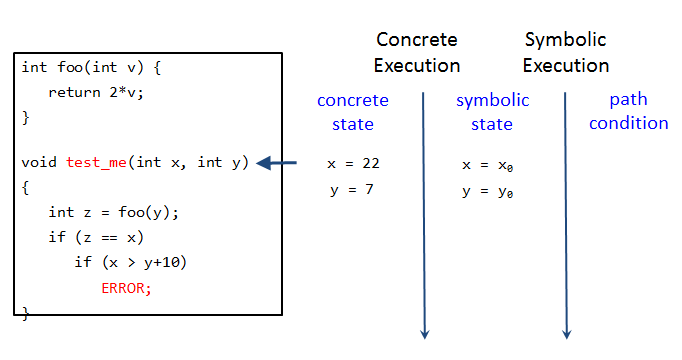
\includegraphics[scale=.7]{dse11.png}
	\end{center}
	\caption{DSE tạo hai đầu vào có giá trị ngẫu nhiên}
	\label{fig:dse11}	
\end{figure}

Ở dòng đầu tiên, $ z $ được gán bằng hàm \texttt{foo(y)}, nghĩa là $ z = 14 $ 
và ở trạng thái biểu trưng của chương trình $ z = 2*y_{0} $ (Hình \ref{fig:dse12}).

\begin{figure}[H]	
	\begin{center}
		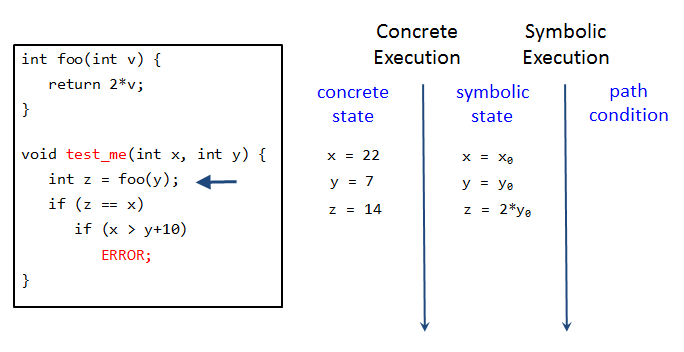
\includegraphics[scale=.7]{dse12.png}
	\end{center}
	\caption{DSE lưu trạng thái biểu trưng của biến $ z = 2*y_{0} $}
	\label{fig:dse12}	
\end{figure}

Tại điểm nhánh $ z == x $, DSE nhận thấy giá trị của $ z = 14$ và $ x = 22 $ 
không bằng nhau, vì vậy DSE lưu lại ràng buộc trong điều kiện đường dẫn của 
chương trình với các giá trị biểu trưng của $ z $ và $ x $ là $ 2*y_{0} != x_{0} $. 
Sau đó, DSE đi theo nhánh \texttt{fasle}, dẫn đến kết thúc chương trình (Hình \ref{fig:dse13}).

\begin{figure}[H]	
	\begin{center}
		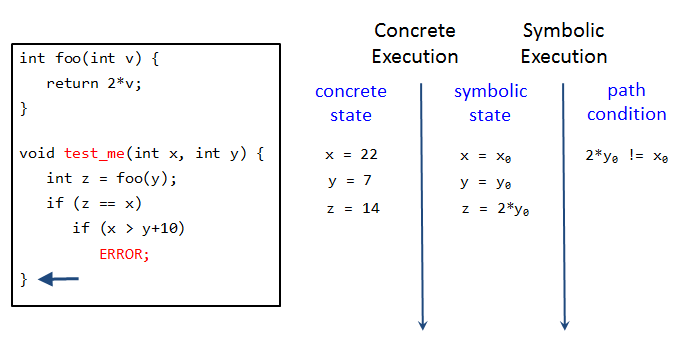
\includegraphics[scale=.7]{dse13.png}
	\end{center}
	\caption{DSE lưu lại ràng buộc của chương trình, $ 2*y_{0} != x_{0} $  }
	\label{fig:dse13}	
\end{figure}

Sau khi kết thúc chương trình, DSE quay trở lại điểm $ z == x $ và chọn nhánh 
\texttt{true}. Để thực hiện việc này, DSE phủ định lại ràng buộc $2*y_{0} != x_{0}$ 
thành $2*y_{0} == x_{0}$. Sau đó, DSE giải ràng buộc $2*y_{0} == x_{0}$ và trả về 
hai số nguyên thỏa ràng buộc có giá trị $ x_{0} = 2$, $ y_{0} = 1 $ (Hình \ref{fig:dse2}).

\begin{figure}[H]	
	\begin{center}
		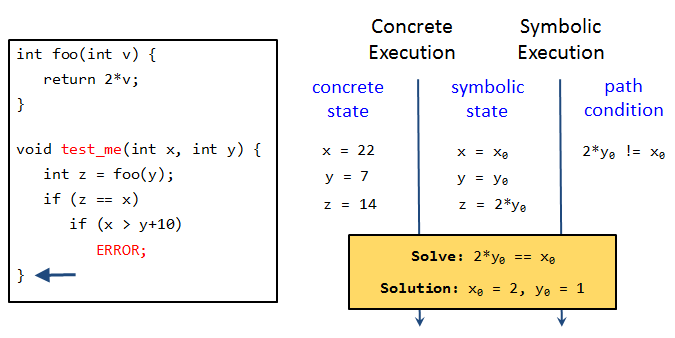
\includegraphics[scale=.7]{dse2.png}
	\end{center}
	\caption{DSE giải ràng buộc $2*y_{0} == x_{0}$}
	\label{fig:dse2}	
\end{figure}

Sau khi có hai số nguyên thỏa ràng buộc của chương trình, DSE khởi động lại hàm 
\texttt{test\_me} với các giá trị đầu vào cụ thể $ x = 2 $, $ y = 1 $ và tiếp tục 
theo dõi trạng thái biểu trưng của chương trình với $ x $ bằng một số $x_{0}$ và 
$ y $ bằng một số $y_{0}$ (Hình \ref{fig:dse21}).

\begin{figure}[H]	
	\begin{center}
		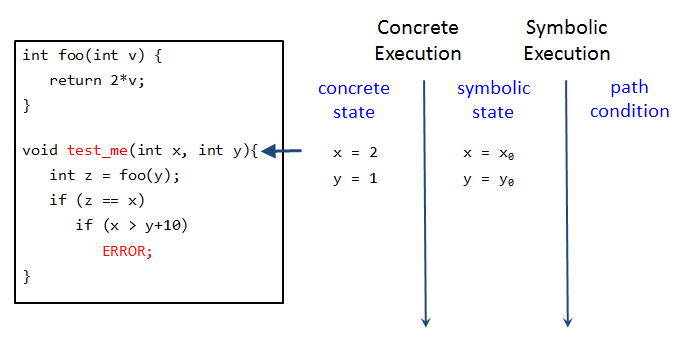
\includegraphics[scale=.7]{dse21.png}
	\end{center}
	\caption{DSE khởi động lại hàm \texttt{test\_me}}
	\label{fig:dse21}		
\end{figure}

Sau khi thực hiện dòng đầu tiên, biến $ z $ sẽ có giá trị bằng $ 2 $ 
(kết quả đầu ra của hàm \texttt{foo(y)}) và DSE lưu giá trị biểu trưng của số 
nguyên $ z $ là $z = 2*y_{0}$ (Hình \ref{fig:dse22}).

\begin{figure}[H]	
	\begin{center}
		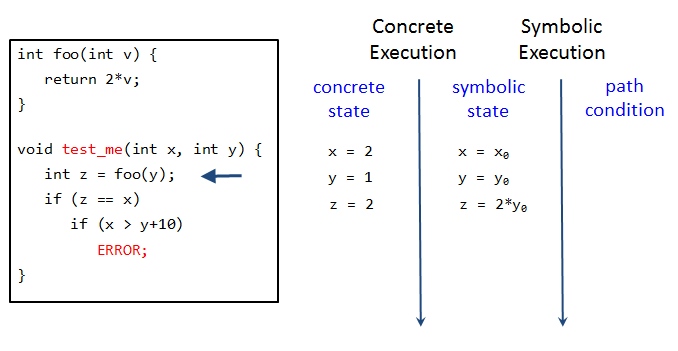
\includegraphics[scale=.7]{dse22.png}
	\end{center}
	\caption{DSE lưu giá trị biểu trưng của số nguyên \texttt{z}}
	\label{fig:dse22}		
\end{figure}

Tại điểm nhánh $ z == x $, DSE thấy giá trị của biến $ z == x $, đây là điều 
kiện \texttt{true} nên DSE lưu lại ràng buộc này trong điều kiện đường dẫn là 
$2*y_{0} == x_{0}$. Sau đó DSE tiếp tục kiểm tra các dòng tiếp theo của nhánh
 \texttt{true} (Hình \ref{fig:dse23}).

\begin{figure}[H]	
	\begin{center}
		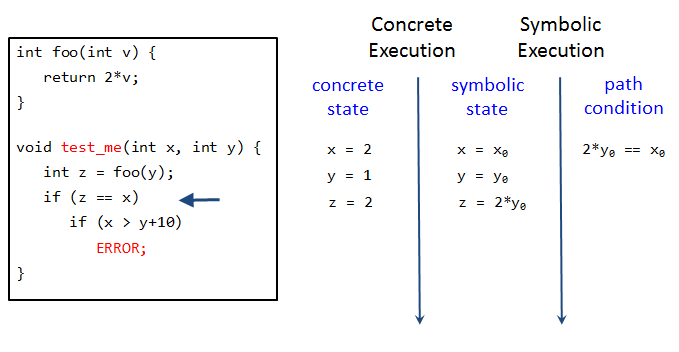
\includegraphics[scale=.7]{dse23.png}
	\end{center}
	\caption{DSE ghi nhận điều kiện ràng buộc $2*y_{0} == x_{0}$}
	\label{fig:dse23}	
\end{figure}

Tại điểm nhánh tiếp theo $ x > y+10 $, lúc này $ x $ có giá trị bằng $ 2 $ 
nhỏ hơn $ (y + 10) $ có giá trị bằng $ 11 $ nên DSE chọn nhánh \texttt{false} 
và kết thúc chương trình. Cùng lúc đó, DSE lưu lại ràng buộc này trong điều 
kiện đường dẫn của chương trình là $x_{0} <= y_{0} + 10$ (Hình \ref{fig:dse24}).

\begin{figure}[H]	
	\begin{center}
		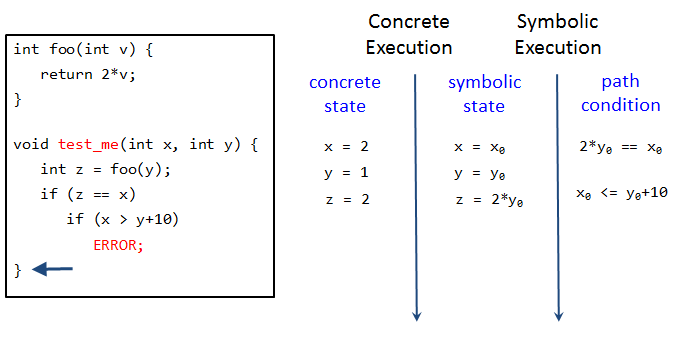
\includegraphics[scale=.7]{dse24.png}
	\end{center}
	\caption{DSE lưu lại ràng buộc $x_{0} <= y_{0} + 10$}
	\label{fig:dse24}		
\end{figure}

Vì đã đến cuối chương trình nên DSE quay lại điểm nhánh $ x > y+10 $ và thực 
hiện phủ định lại ràng buộc $x_{0} <= y_{0} + 10$ thành $ x_{0} > y_{0} + 10 $. 
Sau đó, DSE thực hiện giải ràng buộc $(2*y_{0} == x_{0}) and (x_{0} > y_{0} + 10)$ 
kết quả trả về là $x_{0} = 30$ và $y_{0} = 15$ (Hình \ref{fig:dse3})

\begin{figure}[H]	
	\begin{center}
		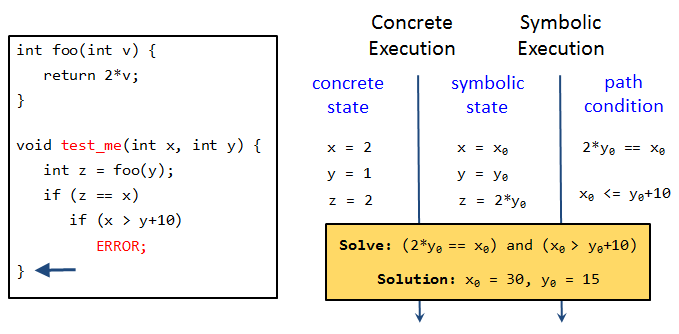
\includegraphics[scale=.7]{dse3.png}
	\end{center}
	\caption{DSE thực hiện giải ràng buộc $(2*y_{0} == x_{0}) and (x_{0} > y_{0} + 10)$}
	\label{fig:dse3}
\end{figure}

Bây giờ, DSE chạy lại hàm \texttt{test\_me} một lần nữa với đầu vào cụ thể $ x = 30 $ 
và $ y = 15 $ và theo dõi trạng thái biểu trưng của chương trình với $x = x_{0}$ 
và $y = y_{0}$ (Hình \ref{fig:dse31})

\begin{figure}[H]	
	\begin{center}
		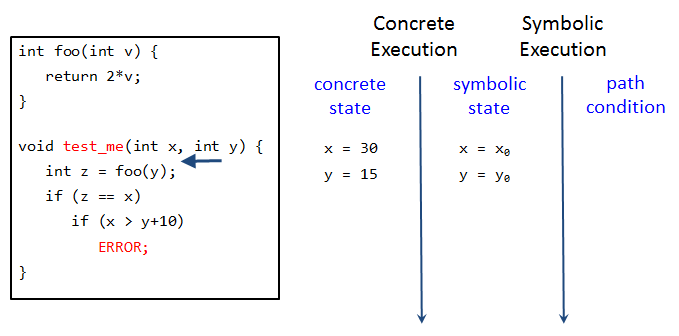
\includegraphics[scale=.7]{dse31.png}
	\end{center}
	\caption{DSE chạy lại hàm \texttt{test\_me} với $ x = 30 $ và $ y = 15 $}
	\label{fig:dse31}
\end{figure}


Ở dòng đầu tiên, số nguyên $ z $ lúc này bằng $ 30 $ và ở trạng thái biểu trưng 
của chương trình, DSE lưu giá trị của số nguyên $ z $ là $ z = 2*y_{0} $ 
như những lần trước đó (Hình \ref{fig:dse32})

\begin{figure}[H]	
	\begin{center}
		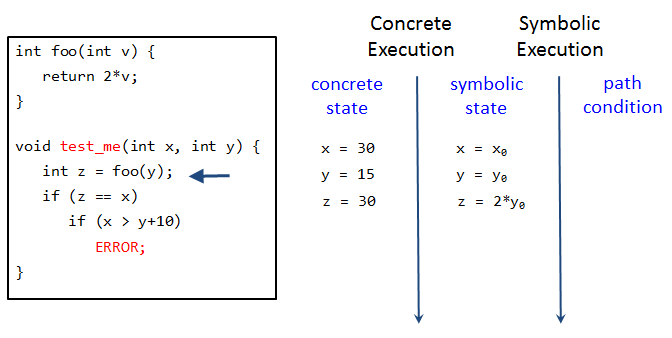
\includegraphics[scale=.7]{dse32.png}
	\end{center}
	\caption{DSE lưu lại trạng thái biểu trưng số nguyên \texttt{z}}
	\label{fig:dse32}
\end{figure}

Tại điểm $ z == x $, DSE nhận thấy giá trị của biến $ z $ bằng giá trị của 
biến $ x $, đây là điều kiện \texttt{true} nên DSE thực thi chương trình 
theo nhánh \texttt{true}, cùng lúc đó DSE lưu lại ràng buộc biểu trưng trong 
điều kiện đường dẫn của chương trình là $ 2*y_{0} == x_{0} $ (Hình \ref{fig:dse33})

\begin{figure}[H]	
	\begin{center}
		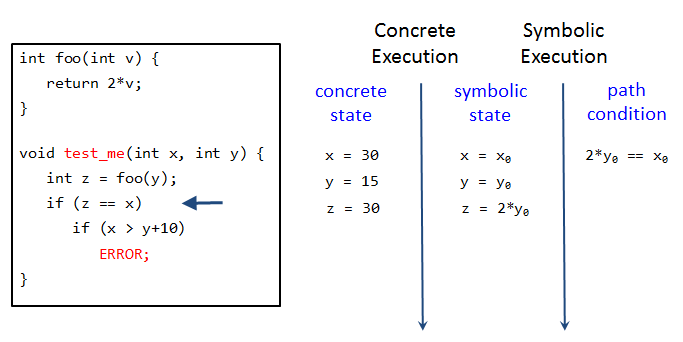
\includegraphics[scale=.7]{dse33.png}
	\end{center}
	\caption{DSE lưu lại điều kiện đường dẫn của chương trình $ 2*y_{0} == x_{0} $}
	\label{fig:dse33}
\end{figure}

Tại điểm nhánh tiếp theo $ x > y+10 $, lúc này giá trị $ x = 30 $, $ y = 15 $ 
nên $ x $ thực sự lớn hơn $ y+10 $, vì vậy DSE thêm một ràng buộc biểu trưng 
mới là $ x_{0} > y_{0}+ 10 $. Nhánh này dẫn đến \texttt{ERROR} và kết thúc chương 
trình nên chúng ta xác định được giá trị đầu vào cụ thể làm cho chương trình 
dẫn đến \texttt{ERROR} là $ x = 30 $ và $ y = 15 $ (Hình \ref{fig:dse4}).

\begin{figure}[H]
	\begin{center}
		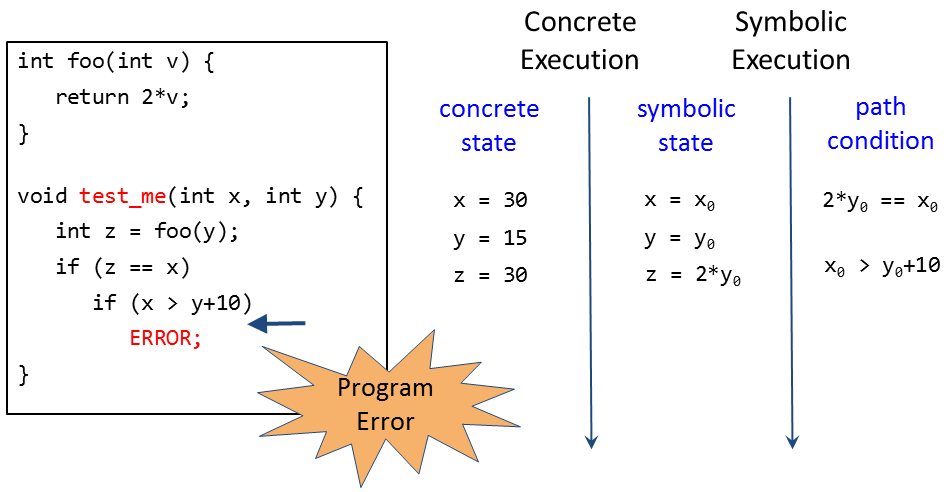
\includegraphics[scale=.6]{dse4.png}
	\end{center}	
	\caption{DSE chạy chương trình với giá trị đầu vào $x = 30$ và $y = 15$}
\label{fig:dse4}
\end{figure}

Tại đây, DSE nhận thấy tất cả các nhánh đường đi trong chương trình đã được 
duyệt nên DSE kết thúc quá trình thực thi. 

Kết quả, sau $ 3 $ lần thực thi chương trình DSE đã tạo ra được các giá trị 
đầu vào $ \{x = 22, y = 7\} $, $ \{x = 2, y = 1\} $ và $ \{x = 30, y = 15\} $, 
các giá trị đầu vào này có thể phủ được tất cả các đường đi của chương trình.
	
\subsection{Một số công cụ áp dụng DSE}	

Trên thế giới hiện có nhiều công cụ sử dụng kỹ thuật DSE để giải quyết
các ràng buộc và tạo ra các giá trị đầu vào có độ phủ cao như như Pex
\cite{tillmann2008pex} và SAGE \cite{godefroid2008automated}\dots và
những công cụ này được phát triển để có thể chạy được trên nhiều nền
tảng khác nhau. Chúng ta có thể tham khảo một số công cụ khác ở Bảng \ref{tbl:DSETools}.
		
\begin{table}[H]
  \centering
  \label{tbl:DSETools}
  \caption{Một số công cụ áp dụng kỹ thuật DSE}
  \begin{tabular} {|c|c|l|}
    \hline 
    \textbf{Tên Công cụ} & \textbf{Ngôn ngữ} & \textbf{Url} \\ 
    \hline 
    KLEE & LLVM & klee.github.io/ \\ 
    \hline 
    JPF	 & Java	& babelfish.arc.nasa.gov/trac/jpf \\
    \hline 
    jCUTE &	Java &	github.com/osl/jcute \\
    \hline 
    JBSE	& Java	 & github.com/pietrobraione/jbse \\
    \hline 
    KeY &	Java &	www.key-project.org/ \\	    
    \hline 
    Otter &	C	& bitbucket.org/khooyp/otter/overview \\
    \hline 
    Rubyx & 	Ruby &	www.cs.umd.edu/~avik/papers/ssarorwa.pdf \\
    \hline 
    Pex	& .NET Framework	 & research.microsoft.com/en-us/projects/pex/ \\
    \hline 
    Jalangi2 &	JavaScript &	github.com/Samsung/jalangi2 \\
    \hline 
    Kite &	LLVM &	www.cs.ubc.ca/labs/isd/Projects/Kite/ \\
    \hline 
  \end{tabular} 
\end{table}
	
\section{Hành vi của chương trình }
\label{sec:behavior}

Trong luận văn này, hành vi của một chương trình là hành động biến đổi
một dữ liệu đầu vào thành đầu ra tương ứng, chương trình được xem như
một hộp đen. Hành vi biến đổi của chương trình từ đầu vào sang đầu ra
là hành động một bước (\emph{one step action/big step}). Nghĩa là ta
không quan tâm đến sự thay đổi của dữ liệu qua từng bước nhỏ khi thực
hiện mỗi câu lệnh trong chương trình mà chỉ xem xét sự thay đổi qua
một bước lớn, xem tất cả các câu lệnh là một câu lệnh ghép.

Để hình thức hóa hành vi của một chương trình và sử dụng trong những
phần tiếp theo, ta tìm hiểu các định nghĩa hình thức liên quan đến
việc thực thi một chương trình, sự tương đương về hành vi giữa hai
chương trình, sự khác biệt về hành vi và độ tương tự về hành vi giữa
hai chương trình \cite{li2016measuring}.
        
\subsection{Thực thi chương trình}

Việc thực thi một chương trình có thể xem là sự tương ứng mỗi giá trị 
vào với một giá trị ra, được nêu ra trong Định nghĩa \ref{def:progexe}.

\begin{definition}[Thực thi chương trình]
  \label{def:progexe}
  Cho $P$ là một chương trình, $I$ là tập hợp các trị đầu vào của $P$
  và $O$ là tập hợp các giá trị đầu ra của $P$. Thực thi chương trình
  P là ánh xạ:
  \[exec: P \times I \rightarrow O.
  \]
\end{definition}

Với giá trị đầu vào $i \in I$, sau khi thực thi chương trình $P$ trên
$i$ ta thu được giá trị đầu ra tương ứng $o \in O, o = exec(P, i)$.

\subsection{Tương đương về hành vi}

Hai chương trình được gọi là tương đương với nhau về hành vi nếu chúng
biến đổi cùng một giá trị vào thành cùng một giá trị ra đối với mọi
giá trị trên miền vào. Xét ví dụ hai chương trình trong Mã lệnh
\ref{lst:SwitchCase} và \ref{lst:IfElse}.

\begin{minipage}[t]{0.45\linewidth}
  \lstinputlisting[label={lst:SwitchCase}, caption =
  {Sử dụng \texttt{switch...case}}]{SwitchCase.cs}
\end{minipage}%
\hfill\vrule\hfill
\begin{minipage}[t]{0.45\linewidth}
  \lstinputlisting[label={lst:IfElse}, caption =
  {Sử dụng \texttt{if...else}}]{IfElse.cs}
\end{minipage}%

Mã lệnh \ref{lst:SwitchCase} và \ref{lst:IfElse} có cùng tham số đầu vào
$ x $ kiểu \texttt{int}, cùng tính toán và trả về giá trị
$ y $ phụ thuộc vào $ x $ theo cách: nếu $ x = 1 $ thì
trả về $ y + 4 $, nếu $ x = 2 $ thì trả về $ 2y $, còn
không thì trả về giá trị bình phương của $ y $.

Rõ ràng hành vi của hai mã lệnh chương trình trên là tương đương vì
chúng trả về giá trị $ y $ giống nhau với cùng mỗi giá trị vào
kiểu số nguyên $ x $, mặc dù chúng có cấu trúc khác nhau (Mã lệnh
\ref{lst:SwitchCase} sử dụng cấu trúc \texttt{switch...case}, Mã lệnh
\ref{lst:IfElse} sử dụng cấu trúc \texttt{if...else} để kiểm tra giá
trị đầu vào $x$). Sự tương đương về hành vi của hai chương trình được
hình thức hóa trong Định nghĩa \ref{def:equiv}.

\begin{definition}[Tương đương về hành vi]
  \label{def:equiv}
  Cho $P_{1}$ và $P_{2}$ là hai chương trình có cùng miền các giá trị
  đầu vào $I$. Hai chương trình này được gọi là tương đương khi và chỉ
  khi thực thi của chúng giống nhau trên mọi giá trị đầu vào trên $I$,
  ký hiệu là exec($P_{1}, I$) = exec($P_{2}, I$).
\end{definition}
	
\subsection{Khác biệt về hành vi}

Dựa vào Định nghĩa \ref{def:equiv} ta có thể suy ra hai chương trình
có hành vi khác nhau nếu chúng có miền giá trị đầu vào khác nhau, hoặc
có một vài giá trị vào làm cho thực thi của chúng khác nhau. Trong
phần này ta chỉ xét những chương trình có cùng miền giá trị vào. 
Ví dụ trong Hình \ref{fig:behavioral-diff} minh họa điều đó.

\begin{figure}[h]
  \centering
  \caption{Ví dụ sự khác biệt về hành vi}
  \label{fig:behavioral-diff}
  \begin{minipage}[t]{0.45\linewidth}
    \lstinputlisting[caption={Khác biệt về hành vi $ P_{1} $}, label={KBHV1}]{Khac_biet_HV_1.cs}
  \end{minipage}%
\hfill\vrule\hfill
\begin{minipage}[t]{0.45\linewidth}
  \lstinputlisting[caption={Khác biệt về hành vi $ P_{2} $}, label={KBHV2}]{Khac_biet_HV_2.cs}
\end{minipage}%
\end{figure}

Trong Hình \ref{fig:behavioral-diff}, hàm $F1$ và $F2$ có cùng miền
giá trị đầu vào kiểu \texttt{int}. Với mỗi giá trị vào \texttt{x}, giá
trị trả về của hàm $F1$ là $x - 10$ và của $F2$ là $x + 10$. Rõ ràng
hai hàm này có hành vi khác nhau. Mô tả hình thức về sự khác biệt hành
vi giữa hai chương trình được nêu ra trong Định nghĩa
\ref{def:equiv-diff}.

\begin{definition}[Sự khác biệt về hành vi]
  \label{def:equiv-diff}
  Cho $P_{1}$ và $P_{2}$ là hai chương trình có cùng miền các giá trị
  đầu vào $I$. Hai chương trình này được xem là có sự khác biệt về
  hành vi khi và chỉ khi thực thi của chúng khác nhau trên một vài giá
  trị đầu vào $i \in I$, ký hiệu là
  $exec(P_{1}, I) \neq exec(P_{2}, I)$.
\end{definition}

\subsection{Độ tương tự về hành vi}

Trong trường hợp hai chương trình không tương đương nhau về hành vi,
nghĩa là có sự khác biệt về hành vi giữa chúng, thì ta cần biết mức độ
tương tự giữa chúng là bao nhiêu. Thông tin này khá hữu ích, nó giúp
cho người dạy có thể đánh giá xếp hạng được giải pháp của người học
dựa vào giải pháp của mình đưa ra, hoặc có thể biết được mức độ hoàn
thiện của giải pháp do người học đưa ra. Xét độ tương tự về hành vi
của hai chương trình $P_{1}$ và $P_{2}$ được cho lần lượt trong Mã
lệnh \ref{TTHV1} và \ref{TTHV2}. Chúng ta dễ dàng thấy được hai hàm
$F1$ và $F2$ là không tương đương nhau trên toàn bộ miền giá trị vào
\texttt{int} mà chỉ tương đương trên miền các giá trị số nguyên
$E = [0,100] \cup \{-1\}$. Từ đó, ta có thể tính được độ tương tự về
hành vi của hai hàm này là $|E| / |\texttt{int}|$, trong đó
$|\mathtt{int}|$ là kích thước miền giá trị vào của hai hàm,
\texttt{int}.

\begin{figure}[H]
	\centering
	\caption{Ví dụ độ tương tự về hành vi}
	\label{fig:behavioral-sim}
	\begin{minipage}[t]{0.45\linewidth}
	  \lstinputlisting[label={TTHV1}, caption = {Chương trình $P_{1}$}]{TuongTu_HV_1.cs}
	\end{minipage}%
	\hfill\vrule\hfill
	\begin{minipage}[t]{0.45\linewidth}
	  \lstinputlisting[label={TTHV2}, caption = {Chương trình  
	    $P_{2}$}]{TuongTu_HV_2.cs}
	\end{minipage}%
\end{figure}

Mô tả hình thức cho độ tương tự về hành vi giữa hai chương trình được
nêu ra trong Định nghĩa \ref{def:equiv-sim}. Trong định nghĩa này,
$I_s$ là tập lớn nhất các giá trị vào mà ở đó hai chương trình tương
đương về hành vi.
    
\begin{definition}[Độ tương tự về hành vi]
  \label{def:equiv-sim}
  Cho $P_{1}$ và $P_{2}$ là hai chương trình có cùng miền giá trị đầu
  vào $I$. Gọi $I_{s} \subseteq I$ là tập con của $I$ sao cho
  $exec(P_{1}, I_{s}) = exec(P_{2}, I_{s})$ và
  $\forall j \in I \setminus I_{s}, exec(P_{1}, j) \neq exec(P_{2},
  j)$. Khi đó, độ tương tự về hành vi giữa $P_1$ và $P_2$ là $|I_s|/|I|$.
\end{definition}

\section*{Tổng kết chương}
 
Chương này tập trung trình bày những định nghĩa liên quan đến hành vi 
của chương trình, độ tương tự về hành vi giữa hai chương trình. 
Ngoài ra, chương này còn cung cấp một số kiến thức cơ sở cho việc 
tìm hiểu những nội dung vừa nêu, cụ thể là kiến thức về kiểm thử phần mềm, 
đặc biệt là kỹ thuật DSE.
 
Thực thi của một chương trình là một ánh xạ tương ứng mỗi giá trị vào
với một giá trị ra. Hành vi của một chương trình được xem xét trong
luận văn này là một hành động một bước, chuyển một giá trị vào thành
một giá trị đầu ra. Khi hai chương trình thực thi giống nhau trên mọi
dữ liệu vào thì chúng được xem là tương đương nhau về hành vi. Ngược
lại, nếu tồn tại một số giá trị vào làm cho chúng thực thi khác nhau
thì được xem là khác biệt về hành vi. Khi hai chương trình không tương
đương về hành vi, ta cần biết chúng tương tự nhau ở mức độ nào thông
qua độ tương tự về hành vi. Để tính độ tương tự giữa hai chương trình
chúng ta có thể đo bằng một trong các phép đo được trình bày trong 
Chương \ref{chap:method}.